\section{Research Outlook}
\label{chap:ourModel}

The standard PFC model doesn't always give satisfying quantitative agreement over a broad range of effects found in real material systems.  The flexibility of the PFC model often means that tuning the model parameters for the accuracy of one of the calculated properties of a material compromises the accuracy of other parameters.  The origin and extent of these limitations isn't well-understood, although various investigations have revealed some clues in terms of the approximations made in the PFC free energy functional \cite{oettel2012description-318, archer2019Deriving, wu2007phasefield-f49, wu2010phasefieldcrystal-7c4} and the dynamics \cite{burns2022timescale-edb}.  The log PFC model addresses some of the concerns raised by Oettel et al. and Archer et al., by explicitly avoiding the fourth-order expansion of the logarithmic term and, as previously shown, opening an additional dimension to the PFC model parameter space.  A number of previously reported PFC results and novel investigations may benefit from the log PFC model, given its greater accuracy and the expanded parameter space it provides.

\subsection{Modeling Real Materials}

The majority of PFC publications focus on qualitative investigations of known effects present in a wide variety of hard and soft condensed matter systems.  There are comparatively few studies that tackle the challenges of qualitatively matching a range of effects for a specific material system \cite{wu2007phasefield-f49, wu2010phasefieldcrystal-7c4}.  Oettel et al. studied a hard sphere model of metallic crystals using density functional theory, with approximations ranging from fundamental measure theory (FMT), to a second-order Taylor expansion of fundamental measure theory (T-DFT), and to a minimal PFC model, which they compared to simulations as a reference \cite{oettel2012description-318}.  The hard sphere model naively describes the interaction between metallic ions as being governed by a potential which is infinite below some distance and zero elsewhere, motivated by the consequences of the Pauli exclusion principle for closed-shell electrons and assuming perfect screening due to the loosely held conducting electrons.  Despite its simplicity, the entropy of packing hard spheres plays a significant role in the surface tension of metallic solids \cite{oettel2012description-318}.  It is also convenient to simulate exactly (SIM), and can be calculated precisely in density field theory via FMT, and approximated via Taylor expansion \cite{oettel2012description-318}.  Their top-line results demonstrated reasonable numeric agreement between SIM and FMT models of the densities within the crystal and liquid surfaces and the surface tension along the three lattice planes of a face-centered cubic FCC crystal and the ratios between them.  For the T-DFT model, they considered two approximations, Percus-Yevick (PY) and White Bear II (WBII), which also gave reasonable agreements for the fluid and crystal densities and lattice plane surface tensions.  Model parameters for the PFC model, which follows from a gradient expansion of the T-DFT (PY) model's pair correlation function, and fourth-order polynomial expansion of the logarithmic term, were selected for the fluid and crystal densities given by the SIM model.  In their derivation of correspondences between model parameters in each of the approximation schemes, they noted an intrinsic problem with the approximations in PFC, which would require $\epsilon$ to have the incorrect sign for consistency with the T-DFT (PY) model and would therefore yield no ordered phases\cite{oettel2012description-318}.  Consequently, they selected a range of $\epsilon$ values from the phase diagram where FCC crystallization would occur, and the resulting surface tensions showed reasonable agreement in ratios between them, but their absolute magnitudes were significantly diminished and heavily dependent upon the choice of PFC temperature \cite{oettel2012description-318}.  Further analysis of the logarithmic PFC model is needed to determine if the source of the $\epsilon$ sign issue is a result of the polynomial expansion, or if instead it is a result of the gradient expansion of the correlation function integrals, which were terminated after fourth-order, the minimum required to produce a PFC crystal with hexagonal symmetry.  Other authors have suggested PFC models with higher-order gradient terms to modify the phase diagram and ground state lattice structure \cite{wu2010phasefieldcrystal-7c4, wu2010controlling-fda, greenwood2011phasefieldcrystal-889}, but no explicit investigations of the role these higher-order terms may play with respect to the temperature model parameter or surface energy are known.

\subsection{Growth on Substrate}

When graphene is grown on a metallic substrate via chemical vapor deposition (CVD), defects and grain boundaries commonly form \cite{huang2011grains-9dd, yu2011control-6aa, song2012origin-9f6}.  Most research on this growth mechanism seeks to grow large sheets of defect-free single crystal graphene for device applications \cite{dai2011rational-807, kim2009largescale-cc6, sun2010growth-dd9}.

However, structural defects in single-layer graphene sheets are of considerable interest in their own right.  For example, single carbon vacancies with and without hydrogen adsorption at the vacancy site are calculated to have magnetic moments of $1\,\mu_B$ and $1.12-1.53\,\mu_B$ respectively, with the latter having a range determined by vacancy concentration \cite{yazyev2007defectinduced-c22}.  Furthermore, these moments produce ferromagnetic or antiferromagnetic coupling depending on which of the two sublattices the vacancies belong to \cite{yazyev2007defectinduced-c22}.  Additional properties of defects in graphene crystals have been studied, particularly on metal substrates, for example \cite{ugeda2011point-033, lahiri2010extended-120}, as well as commensurate measures to engineer these defects into the graphene lattice \cite{lahiri2010extended-120}.  

In Ref.~\cite{niu2013growth-4f5}, T. Niu et al. used low-temperature scanning tunneling microscopy (LS-STM) to image the CVD deposition growth stages on Cu(111) facets.  Their samples were grown by thermal decomposition of methane under vacuum over a series of cycles of exposure at room temperature, followed by annealing at $800\,^\circ$C.  Though their goal was to produce large defect-free sheets of graphene, their method resulted in an intermediate stage which they called "defective graphene", exhibiting pseudoperiodic corrugations and pseudo-ordered point defects (vacancies).  Fig.~\ref{fig:defect-graphene} from \cite{niu2013growth-4f5} shows STM images of a defective graphene crystal exhibiting a diamond-shaped moir\'e unit cell with dimensions of $\sim6.0$ nm per side.  Corrugation, due to lattice mismatch between graphene and the substrate, is present along the edges and through the shorter body diagonal, indicated with a cyan arrow.  The close-up in panel (b) shows three vacancy defects surrounding the vertex where four unit cells meet.

Two additional studies demonstrate the potential for substrate lattice mismatch to provide a controllable mechanism for producing graphene sheets with engineered structural defects.  In Ref.~\cite{lahiri2010extended-120}, they used an Ni(111) substrate to realize a one-dimensional defect comprised of a regular arrangement of octagonal and pentagonal carbon rings.  The regularity of the defect line was due to two distinct ways in which graphene could grow on the substrate that had a relative translation of $1/3(\vec{a}_1 + \vec{a}_2)$, where $\vec{a}_1$ and $\vec{a}_2$ are the unit cell vectors vectors, resulting in a dislocation along the $\vec{a}_1 - \vec{a}_2$ direction.  Another example was realized on Pt(111), wherein vacancy defects were generated on an initially perfect crystal by irradiating with Ar$^+$ ions.  The vacancies preferentially form where carbon atoms are relatively weakly bonded due to the underlying moir\'e pattern induced by the substrate \cite{ugeda2011point-033}.

Due to the aforementioned novel properties of structural defects in graphene and the dependence of the location of these defects on particular sublattices, the ability to produce regular patterns of defects within the graphene lattice may be of considerable interest.  Furthermore, the log PFC model could be well-suited to predict such pattern formation for epitaxial growth on a mismatched substrate, particularly by extending log PFC with out-of-plane height deformations, which would enable modeling both observed effects, namely corrugation and point defect formation.  An additional line of inquiry would be to calculate the PFC bond strength in the resulting graphene sheet to predict which carbon atoms would be most likely to be removed by Ar$^+$ irradiation, as in Ref.~\cite{ugeda2011point-033}.

\begin{figure}[!htbp]
    \centering
    \begin{subfigure}[t]{0.85\linewidth}
        \centering
        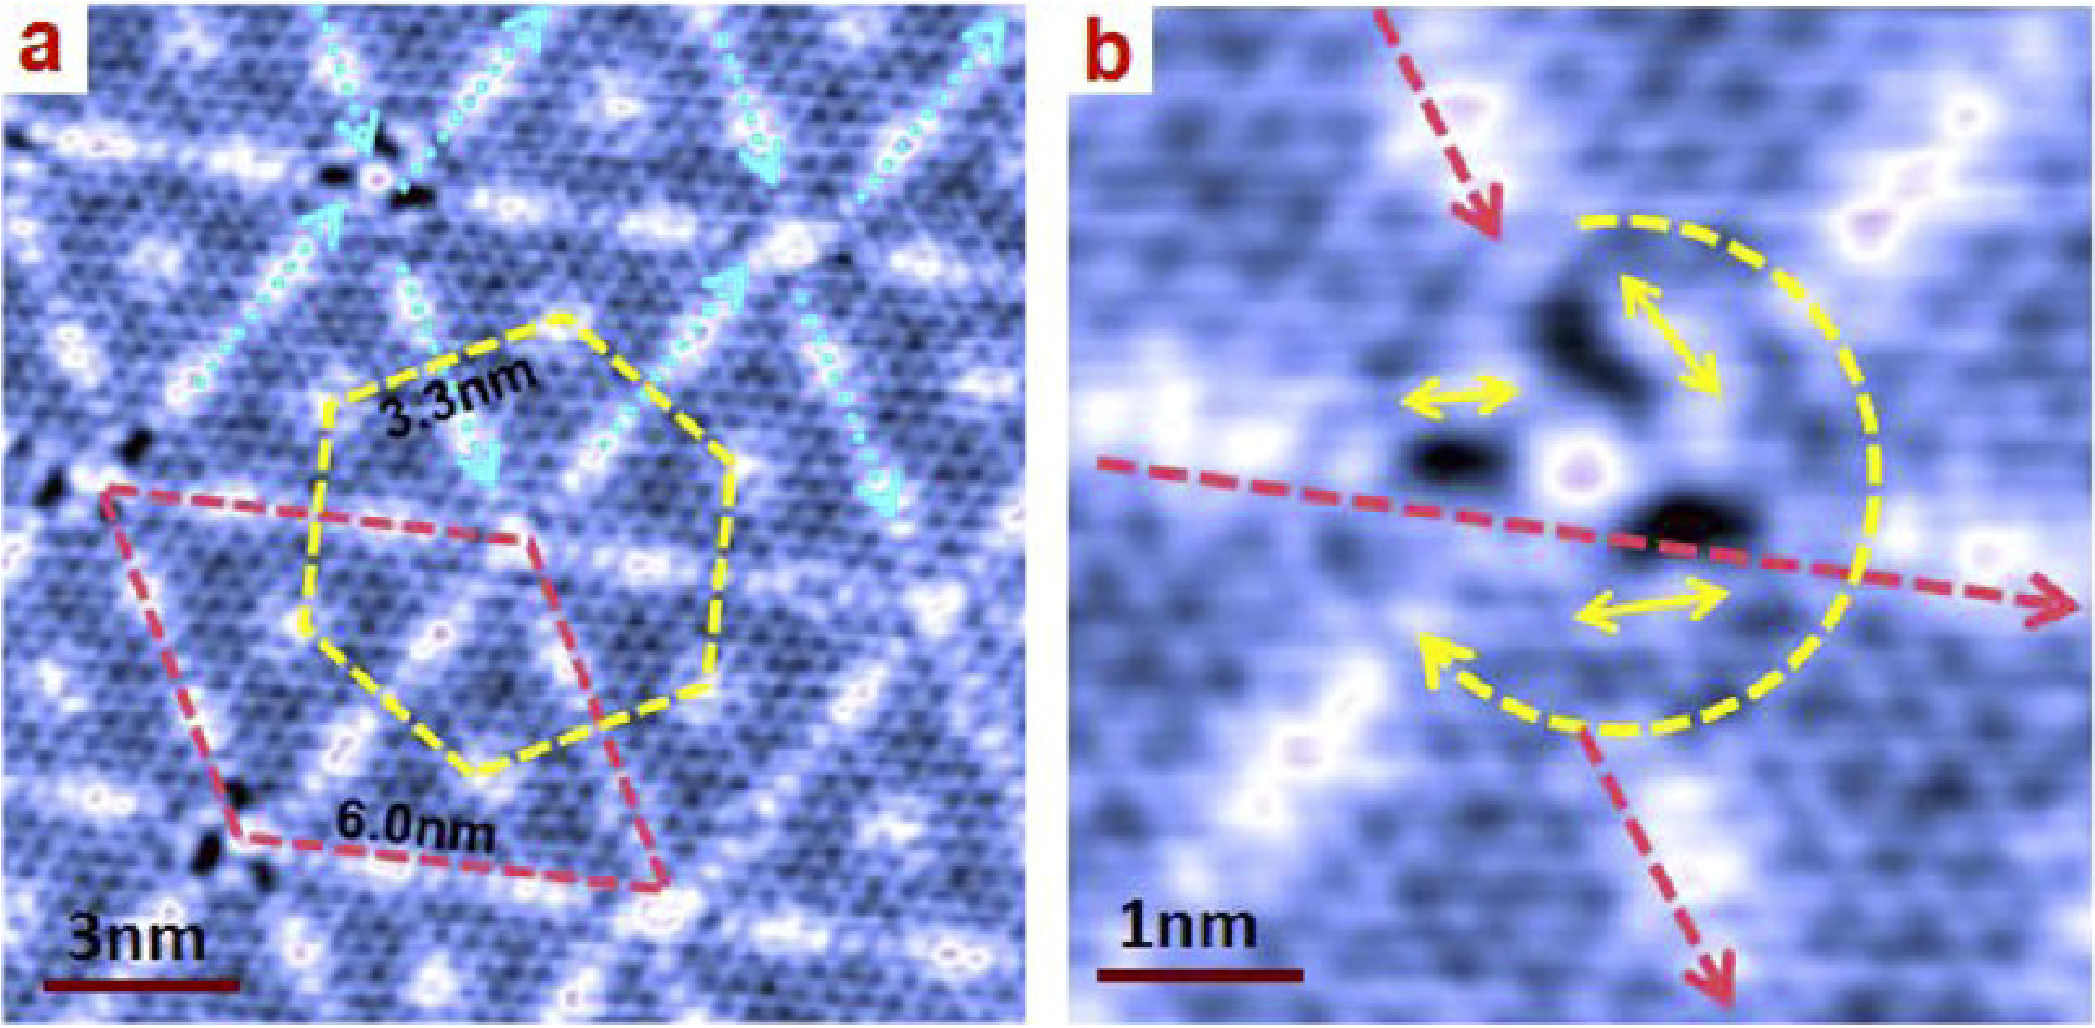
\includegraphics[width=\linewidth]{fig/fig-defect-graphene.png}
    \end{subfigure}
    \caption{Figure 5 from \cite{niu2013growth-4f5} showing STM image of defective graphene with pseudoperiodic corrugation and vacancies.  In panel (a), the red diamond marks the unit cell.  Vacancies were often observed at the vertices of unit cells.  The yellow hexagon indicates the nearest neighboring vacancy-free moir\'e spot.  The green arrows indicate corrugation folds.  Panel (b) is a close-up image of the vacancies commonly found at unit cell vertices, which formed at the terminus of the corrugations. }
    \label{fig:defect-graphene}
\end{figure}

\FloatBarrier
\subsection{Plasticity and the Portevin-Le Chatelier (PLC) Effects}
The deformation of solid materials is characterized by two effects.  The first effect is elastic deformation, in which the shape of a body changes in response to external forces like compression, tension, or shear forces, and relaxes to the initial state when the external force is removed.  Appendix \ref{appendix:oddElasticity} provides a general theory of elasticity following the development of Landau and Lifshitz \cite{landau2012theory}.  In a purely elastic deformation, chemical bonds are strained but not broken.  The second effect is plastic deformation, wherein the shape of the body is permanently altered due to rearrangements of the atoms, the breaking of some bonds, and the formation of new bonds.  The theory of plastic deformations is not as well defined and tends to rely on phenomenological descriptions of specific materials (see Ashcroft and Mermin \cite{ashcroft_mermin_1976_ch30} for a general description or Marder \cite{marder_2000_ch15_title} for a fluid dynamics description of plasticity).  Practically, plasticity is often exhibited in metals and can be understood as the ability to reshape a metal, typically by heating the metal to soften the material and hammering, bending, rolling, or stamping to achieve a new physical form.  A microscopic description of plastic deformations in metals is complex and involves the flow of dislocations into the body while under strain ~\cite{marder_2000_ch15_title}.  In real materials, the degree of strain required to achieve plastic deformations is high relative to elastic strain, but orders of magnitude lower than idealized models that treat bodies as perfect crystals and treat the metallic bonds as Hookean springs \cite{ashcroft_mermin_1976_ch30}.  In large part, this is due to the fact that most metallic solids contain high densities of dislocations and stacking faults, resulting in an intrinsic strain within the body of metal that facilitates the bond breaking associated with plastic deformations.  Repeated plastic deformations also introduce new dislocations into the body, which initially can further soften the material, but over time tend to make the material more stiff and prone to cracks (as in bending a wire back and forth repeatedly until it eventually breaks).  This is known as work hardening and is due to the accumulation of complex defect structures beyond simple dislocations.  While some dislocation defects often soften a crystal, the mechanical work required to break bonds in highly defective crystals can increase substantially \cite{ashcroft_mermin_1976_ch30}.

In two-dimensional PFC models, it is possible to investigate plastic deformations and related dynamics in a number of ways.  For example, it is possible to introduce strain into the simulated system via opposing advective density flows across regions of a PFC crystal.  The strength of the advective flow required to cause plastic deformations can be determined by simulation and used to derive the yield stress.  The PFC crystals can be either perfect crystals or crystals with various types of defects introduced into the lattice, including grain boundaries, line dislocations, or vacancies.  The accumulation of stress within the crystal can be calculated as changes to the free energy, and the dynamics of plastic reformation and relaxation can be observed as the PFC atoms move to neighboring lattice sites.  Additionally, changes to elasticity can be measured as a function of the type and quantity of accumulated defects in the system, as well as changes to the yielding stress for plastic deformations, thus permitting the study of work hardening.  In real two-dimensional systems, strain is often associated with lattice mismatch between the 2D material and the substrate on which it was grown.  Thus, graphene grown on a piezoelectric substrate allows the amount of strain induced on the graphene layer to be controlled by an external electric field \cite{gonzález2017manybody-4d0}.  Similar effects could be modeled in PFC by introducing a periodic potential to represent the substrate and modifying the spacing of this potential during the simulation to create similar effects. 

The Portevin-Le Chatelier (PLC) effect describes the uneven, "jerky" nature exhibited by some materials as they undergo plastic deformations.  The source of the effect has been attributed to pinning effects at defect cores within the body of the material, and the subsequent breaking free of this pinning \cite{abbadi2002characteristics-943}.  In a stress versus strain plot, the PLC effect exhibits a sawtooth structure as depicted in Fig.~\ref{fig:sawtooth}.  In their paper \cite{chan2010plasticity-49d}, Chan and Goldenfeld et al. investigated the breaking free of accumulated strain in crystals with varying defect landscapes, a process they referred to as an avalanche event.  From their measurements, they extracted a critical exponent for the probability of such a collapse in the stress as a function of the shear rate and found agreement with experiment and mean field theory predictions.  The vacancy diffusion results shown in Fig.~\ref{fig:diffusion-sawtooth} (same as Fig.~\ref{fig:vacancy-diffusion}, with hand-drawn lines added to illustrate the semblance of a sawtooth wave) show the average mean square displacement of ten independent log PFC simulations for each value of $\eta$ investigated, and suggest a similar sawtooth structure over multiple periods of vacancy diffusion, particularly evident at the lowest level of thermal noise investigated ($\eta_0 = 0.15$).  The stability of log PFC atoms and vacancies with respect to fluctuations in density was used as a criterion to find appropriate model parameters to perform these studies, although a unified concept of temperature that incorporates the impact of the model parameter $\epsilon$ and the magnitude of thermal noise $\eta_0$ has yet to be established, and a convenient metric for what is meant here by vacancy stability has not been formally defined.  Nonetheless, this author's investigations of vacancy diffusion in the standard PFC model so far suggest that the standard PFC parameters necessary to give rise to vacancy stability in terms of their robustness against unintended formation or annihilation caused by density fluctuations limit the magnitude of thermal fluctuations that can be introduced into the system, such that diffusion is either too slow to observe or nonexistent.  Though not conclusive, this seems to indicate a "stiffness" in the structure of the log PFC atom that can be tuned independently from the energetic barrier to vacancy diffusion.

\begin{figure}[!htbp]
    \centering
    \begin{subfigure}[t]{0.85\linewidth}
        \centering
        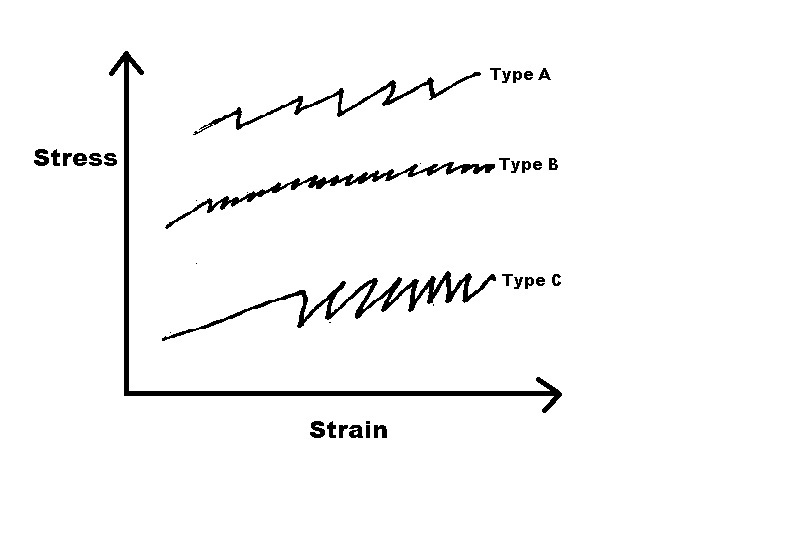
\includegraphics[width=\linewidth]{fig/Serration_types.jpg}
    \end{subfigure}
    \caption{Wikicommons (https://commons.wikimedia.org/wiki/File/Serration\_types.jpg) depiction of various stress-strain sawtooth bands showing a common classification schema.}
    \label{fig:sawtooth}
\end{figure}

\begin{figure}[!htbp]
    \centering
    \begin{subfigure}[t]{0.85\linewidth}
        \centering
        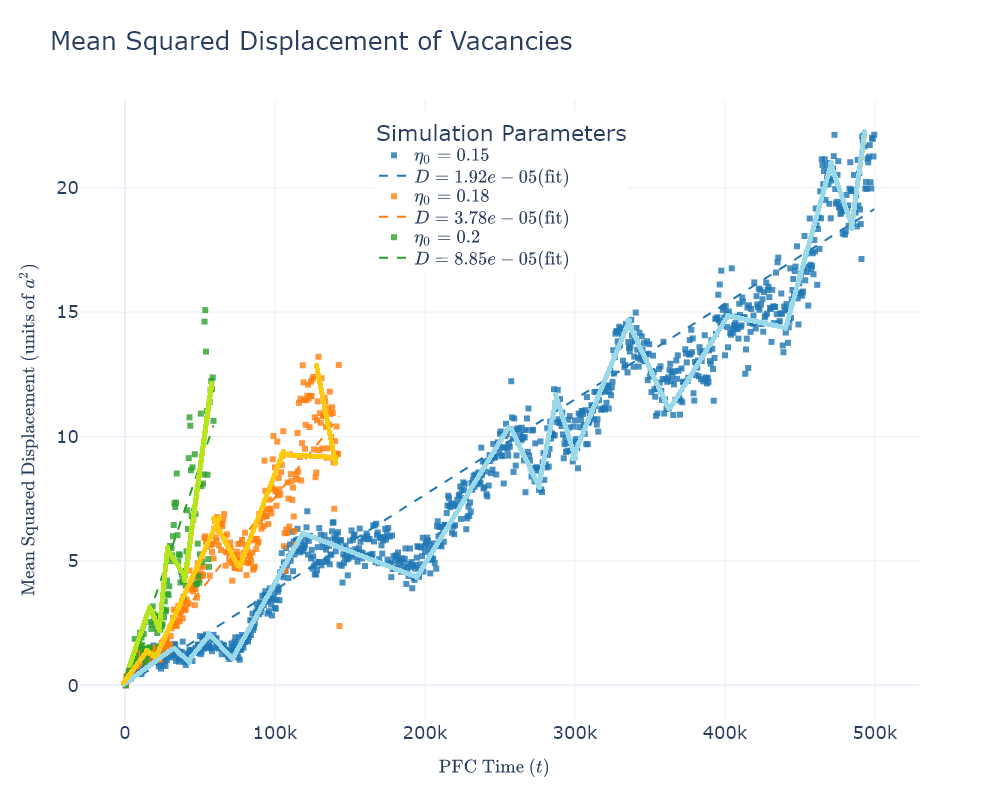
\includegraphics[width=\linewidth]{fig/fig-vacancy-diffusion-eta-sawtooth.png}
    \end{subfigure}
    \caption{Vacancy diffusion suggestive of the jerky behavior of pinning and depinning.}
    \label{fig:diffusion-sawtooth}
\end{figure}

\FloatBarrier
\subsection{Active Matter Crystal Edge Currents}

Active matter broadly concerns the behavior of systems in which the constituent components of the system are capable of self-propulsion --- i.e., converting an environmental energy source into mechanical motion.  Nature provides numerous examples of active matter systems across a wide range of length scales, from the flocking behavior of birds or the schooling of fish, to rafts of organisms such as starfish embryos or mobile bacteria, down to biologically active molecules such as actin or motor proteins.  Researchers have also created artificial active matter using swarms of simple machines or Janus particles. Active systems, by their nature, are out of equilibrium in a thermodynamic sense, although many active systems exhibit some of the same behaviors associated with passive condensed matter systems in thermodynamic equilibrium, including symmetry breaking via periodic arrangements and stable phase separation.  However, active systems can also exhibit exotic behaviors such as odd elasticity (see Appendix~\ref{appendix:oddElasticity}), spontaneous rearrangements, and non-Newtonian dynamics.  PFC models have already been altered to incorporate non-reciprocal interactions, and subsequent simulations have replicated several of the dynamics observed in biological and artificial systems.

In Ref.~\cite{huang2025anomalous}, Huang et al. developed a PFC model that incorporated transverse forces between PFC atoms and calculated the odd bulk modulus $A$ and odd shear modulus $K^\circ$ in terms of newly introduced model parameters.  Through simulations, they demonstrated that their active PFC model exhibited a mixture of behaviors associated with passive systems, such as crystal nucleation, and behaviors that were purely active, such as self-rotation and self-fission of the odd crystal \cite{huang2025anomalous}.  Similar behaviors have been observed in active crystals comprised of many individual organisms, including starfish embryos \cite{tan2022odd} and bacteria \cite{petroff2015fast}, both of which self-organize into crystals due to hydrodynamic interactions caused by rapid spinning at a confined surface.  However, one dynamic observed by Petroff et al. in the spinning bacteria, namely, a surface current of bacteria that rotated around the bulk of the active crystal, was not observed in PFC simulations.  Petroff et al. calculated the edge current's dependency on the size of the crystal and the number of elements on the crystal edge.  Overall system stability was heavily dependent on whether the number of elements was consistent with perfectly hexagonal crystals, with crystals missing a single element or having one extra element exhibiting the greatest instability.  In Fig.~\ref{fig:edge-current} panel (a), a full hexagonal crystal is shown and rotates uniformly.  In panel (b), the outermost ring is missing one spinner and the vacancy moves counter to the crystal rotation as spinners hop one-by-one into the vacancy position.  In panel (c), an extra spinner is free to move independently, and thus faster, along the outer edge of the crystal.

Depending on the number of bacteria, Petroff et al. calculated that the edge currents could be faster, slower, or roughly the same as the crystal's natural rotation, and confirmed these calculations experimentally by manually manipulating small rafts of bacteria spinners \cite{petroff2015fast} (see supplemental movies).  The active PFC model due to Huang et al., however, produced odd crystals with diffusive borders and thus an indefinite number of elements.  Consequently, no evidence of edge currents was reported \cite{huang2025anomalous}.  Modeling such behavior likely requires that the edges of the odd crystal be sufficiently sharp, with discrete rather than diffuse PFC atoms along the edge, so that the system can be simulated with a precise number of elements in order to replicate the edge behaviors of the natural crystal observed by Petroff et al.  While it may be possible to achieve the requisite sharpness in an active-standard PFC model, an active-log PFC model will widen the range of parameter space that can be explored and may prove to be more suitable for replicating edge effects and other tangible behaviors, including the behavior of vacancies in the odd crystal.

\begin{figure}[htbp]
  \centering
  \begin{tikzpicture}
    % Load the PDF as a node so we can overlay labels precisely.
    % Adjust width as needed (here: 0.9\textwidth).
    \node[inner sep=0] (img) {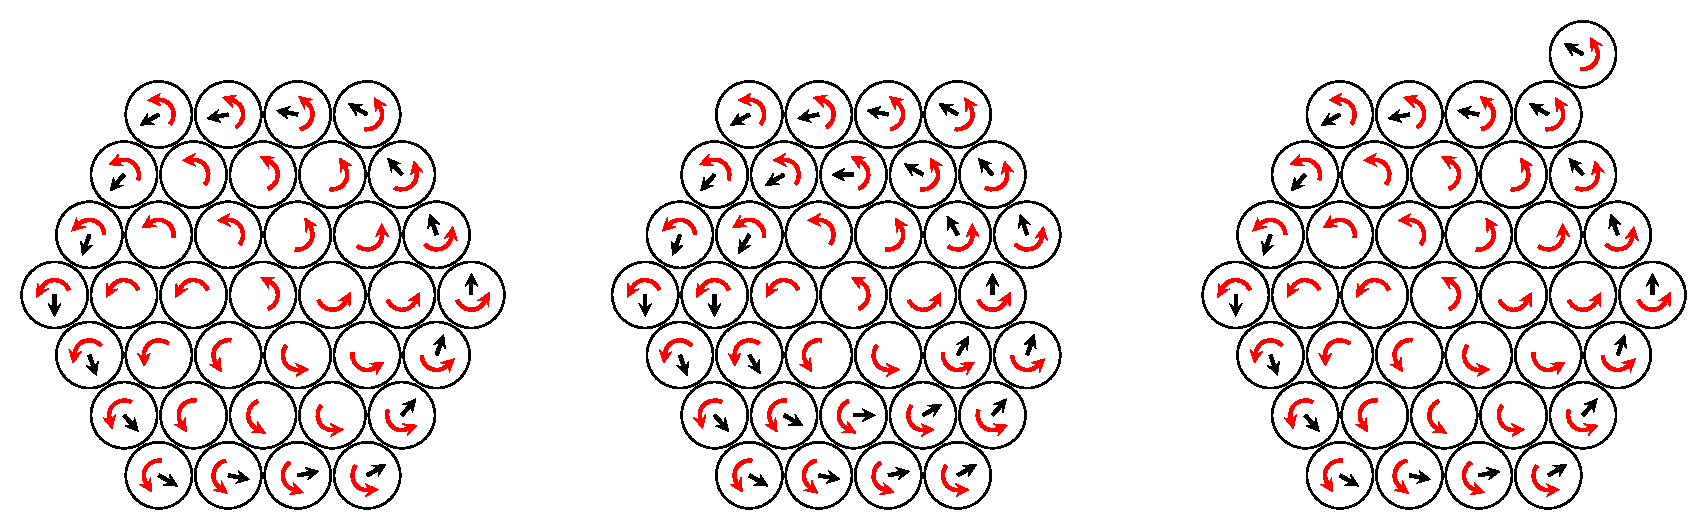
\includegraphics[width=0.9\textwidth]{fig/fig-edge-current.pdf}};

    % Compute three positions along the top edge of the image.
    % pos values (0.18, 0.50, 0.82) are tuned to sit above the three subfigures;
    % tweak them if your PDF layout differs slightly.
    \path (img.north west) -- (img.north east) coordinate[pos=0.18] (labA);
    \path (img.north west) -- (img.north east) coordinate[pos=0.50] (labB);
    \path (img.north west) -- (img.north east) coordinate[pos=0.82] (labC);

    % Vertical offset above the image (increase to move labels farther up)
    \def\labelVoffset{6mm}

    % Labels (bold). Change text as desired.
    \node[font=\bfseries, anchor=south] at ($(labA)+(0,\labelVoffset)$) {19 spheres (R=4)};
    \node[font=\bfseries, anchor=south] at ($(labB)+(0,\labelVoffset)$) {18 spheres (R=4 -1)};
    \node[font=\bfseries, anchor=south] at ($(labC)+(0,\labelVoffset)$) {20 spheres (R=4 +1)};

    % Optional: small subcaptions under each subfigure (uncomment and edit)
    \node[font=\small, anchor=north] at ($(labA)+(-30pt,5pt)$) {(a)};
    \node[font=\small, anchor=north] at ($(labB)+(-20pt,5pt)$) {(b)};
    \node[font=\small, anchor=north] at ($(labC)+(-10pt,5pt)$) {(c)};

  \end{tikzpicture}
  \caption{Edge current configurations:  Red arrows indicate the direction of spin.  Black arrows show the net force acting on each spinner.  If the longitudinal force is sufficiently large compared to the transverse force, the crystal remains intact.  In (a) the whole crystal rotates uniformly.  In (b), the outer edge rotates around the crystal by the spinner before the vacancy hopping into the vacancy position.  After each hop, the next spinner before the vacancy hops, establishing a counter-rotation of the vacancy, i.e. the hopping rotation is slower than the overall crystal rotation.  In (c), the extra spinner is free to move around the edge and moves faster than the crystal rotation.}
  \label{fig:edge-current}
\end{figure}

\FloatBarrier
\subsection{Summary}

PFC models provide a foundation for exploring many material properties across a wide range of material systems.  They are built upon a straightforward mathematical description derivable from classical DFT that captures the essential behavior of more complex models, while being computationally convenient.  They allow for the exploration of microscopic details at diffusive timescales, bridging the gap between the extremes of groundstate accuracy provided by classical DFT and the detail of trajectories provided by MD simulations.  Despite numerous successes over the previous two decades, a number of challenges regarding the ability of PFC models to serve as a general model for crystalline solids have been reported, with many remaining unaddressed.  The logarithmic PFC, by maintaining a more accurate description of the theoretical frameworks that underpin the PFC model, may hold promise for greater accuracy with the same degree of microscopic detail and over the same diffusive timescales as the standard PFC model.  As noted, logarithmic PFC restores a potentially useful dimension of the PFC parameter space lost by the standard PFC's Taylor expansion of the log term.  The retention of the log term has already been demonstrated to be useful with respect to stabilizing vacancies, and while vacancy stabilization was previously overlooked in the standard PFC model, it has been demonstrated that the expanded parameter space in log PFC was useful in studying MD-like vacancy diffusion in PFC.  Additional theoretical and numerical analysis will help quantify the differences in behavior between log PFC and standard PFC models, and enumerate the impacts of the larger parameter space of the latter.  The impact on the landscape of PFC applications may be broad, with potential impacts on the microscopic details of 2D crystals grown on substrates, the evolution of the strain-stress relationships during plastic deformations, and greater detail for active matter systems, especially at surface boundaries, having been previously noted.  Realization of these benefits, and potentially many more, seems within grasp and makes log PFC a potentially exciting model for the future.